%% LaTeX-Beamer template for KIT design
%% by Erik Burger, Christian Hammer
%% title picture by Klaus Krogmann
%%
%% version 2.1
%%
%% mostly compatible to KIT corporate design v2.0
%% http://intranet.kit.edu/gestaltungsrichtlinien.php
%%
%% Problems, bugs and comments to
%% burger@kit.edu

\documentclass[18pt]{beamer}

\usepackage[utf8]{inputenc}
\usepackage[babel,german=quotes]{csquotes}
\usepackage{graphicx}
\usepackage{caption}
\usepackage{subfig}
\usepackage[right]{eurosym}
\usepackage{listings}


\usepackage{amssymb} % for |N
\newcommand{\Hilight}{\makebox[0pt][l]{\color{cyan}\rule[-4pt]{0.65\linewidth}{14pt}}}	%from http://newsgroups.derkeiler.com/Archive/Comp/comp.text.tex/2008-10/msg00877.html


%% SLIDE FORMAT

% use 'beamerthemekit' for standard 4:3 ratio
% for widescreen slides (16:9), use 'beamerthemekitwide'

\usepackage{templates/beamerthemekit}
% \usepackage{templates/beamerthemekitwide}

%% TITLE PICTURE

% if a custom picture is to be used on the title page, copy it into the 'logos'
% directory, in the line below, replace 'mypicture' with the 
% filename (without extension) and uncomment the following line
% (picture proportions: 63 : 20 for standard, 169 : 40 for wide
% *.eps format if you use latex+dvips+ps2pdf, 
% *.jpg/*.png/*.pdf if you use pdflatex)

\titleimage{title}

%% TITLE LOGO

% for a custom logo on the front page, copy your file into the 'logos'
% directory, insert the filename in the line below and uncomment it

\titlelogo{titlelogo}

% (*.eps format if you use latex+dvips+ps2pdf,
% *.jpg/*.png/*.pdf if you use pdflatex)

%% TikZ INTEGRATION

% use these packages for PCM symbols and UML classes
% \usepackage{templates/tikzkit}
% \usepackage{templates/tikzuml}

% the presentation starts here

\title[C++ Workshop]{C++ Workshop}
\subtitle{2. Block, 04.05.2012}
\author{Robert Schneider}

\institute{}

\begin{document}

% change the following line to "ngerman" for German style date and logos
\selectlanguage{ngerman}

\AtBeginSection[]{%
	\begin{frame}
		\tableofcontents[sectionstyle=show/hide,subsectionstyle=hide/show/hide]
	\end{frame}
	\addtocounter{framenumber}{-1}% If you don't want them to affect the slide number
}

%title page
\begin{frame}
\titlepage
\end{frame}

%table of contents
\begin{frame}{Gliederung}
\tableofcontents
\end{frame}

%%%%%%%%%%%%%%%%%%%%%%%%%
% ADD OWN SECTIONS HERE %
%%%%%%%%%%%%%%%%%%%%%%%%%
\section{C++}


\begin{frame}{Was ist C++?}
	\begin{block}{Eine standardisierte Programmiersprache}
		C++
		\begin{itemize}
			\item ist eine Programmiersprache (gibt einen Programmablauf vor)
			\item vereint sowohl high-level- wir auch low-level-Features
			\item ist sehr hardwarenah
			\item ist standardisiert (\emph{hier:} ISO/IEC 14882:2003)
		\end{itemize}
	\end{block}
	
	\pause
	
	\begin{block}{Was sagt der Standard hierzu?}
		C++ is a general purpose programming language based on the C programming language as described in
		ISO/IEC 9899:1990 Programming languages – C.
	\end{block}
\end{frame}

\begin{frame}{Worum geht es bei C++?}
	von-Neumann-Architektur $\xrightarrow{Abstraktion}$ C++ $\xrightarrow{Implementierung}$ Hardware
	
	\begin{itemize}
		\item C++ wurde explizit für die von-Neumann-Architektur designed
		\item C++ soll zero-overhead sein (Features, die ich nicht nutze, benötigen weder Speicher noch Laufzeit)
		\item C++ ist eine Multi-Paradigmen-Sprache mit Betonung der Objektorientierung
	\end{itemize}
	
	\begin{block}{Standard, 1.8}
		The constructs in a C++ program create, destroy, refer to, access, and manipulate objects.
	\end{block}
\end{frame}

\begin{frame}{Wofür nutze ich C++?}
	foo!
\end{frame}

\begin{frame}[fragile]{»Dinge«}
	Das grundlegende Konzept in C++ nennt sich im Standard \enquote{object}. Hinsichtlich Java und Objektorientierung aber missverständlich!
	Wir nennen es daher »Ding«.
	
	\pause
	
	\small
	\begin{block}{Standard, 1.8}
		Ein »Ding«
		\begin{itemize}
			\item ist ein Speicherbereich, aber \emph{keine} Funktion (auch wenn diese Speicher belegt!).
			\item wird durch eine Definition, den \verb|new|-Ausdruck oder vom Compiler erzeugt.
			\item hat einen Typen und eine Speicherdauer {\tiny (die die Lebensdauer des dort gespeicherten »Objekts« beeinflusst)}; \emph{kann} einen \emph{Namen} haben.
			\item hat eine Größe von einem oder mehr Bytes {\tiny (abgesehen von bit-fields)}.
			\item von »einfachem« {\tiny (POD)} Typ besetzt eine zusammenhängende Menge Bytes.
		\end{itemize}
	\end{block}
\end{frame}

\begin{frame}[fragile]{Speicher}
	\begin{block}{Standard, 1.7}
		Die fundamentale Speicher-Einheit im C++ Speichermodell ist das \emph{Byte}. [Es folgt eine sehr abstrakte Definition.]
		Der Speicher, welcher einem C++ Programm zur Verfügung steht, besteht aus einer oder mehreren Sequenzen von zusammenhängenden Bytes.
		Jedes Byte hat eine eindeutige Adresse.
	\end{block}
	
	\footnotesize
	\begin{block}{}
		\begin{lstlisting}[language=C++]
			int foo;
			int bar;
			double d;
			double& rd = d;
			
			cout << sizeof(foo);
			cout << sizeof(int);
		\end{lstlisting}
	\end{block}
\end{frame}

%, memory model, object model, Ring HW-Standard-Impl
\section{»Dinge«, Referenzen und Pointer}


\subsection{»Dinge« und Speicher}

\begin{frame}[fragile]{»Dinge«}
	Das grundlegende Konzept in C++ nennt sich im Standard \enquote{object}. Hinsichtlich Java und Objektorientierung aber missverständlich!
	Wir nennen es daher »Ding«.
	
	\pause
	
	\begin{block}{Standard, 1.8}
		Ein »Ding«
		\begin{enumerate}
			\item ist ein Speicherbereich, aber \emph{keine} Funktion {\tiny(auch wenn diese Speicher belegt!)}.
			\item hat eine Speicherdauer, einen Typen und \emph{kann} einen \emph{Namen} haben.
			\item {\scriptsize hat eine Größe von einem oder mehr Bytes {\tiny (abgesehen von bit-fields)}.}
			\item {\scriptsize von »einfachem« {\tiny (POD)} Typ besetzt eine zusammenhängende Menge Bytes.}
			\item {\scriptsize wird durch eine Definition, den \verb|new|-Ausdruck oder vom Compiler erzeugt.}
		\end{enumerate}
	\end{block}
\end{frame}

\begin{frame}[fragile]{Speicher}
	\begin{block}{Standard, 1.7}
		Die fundamentale Speicher-Einheit im C++ Speichermodell ist das \emph{Byte}. [Es folgt eine sehr abstrakte Definition.]
		Der Speicher, welcher einem C++ Programm zur Verfügung steht, besteht aus einer oder mehreren Sequenzen von zusammenhängenden Bytes.
		Jedes Byte hat eine eindeutige Adresse.
	\end{block}
	
	\pause
	
	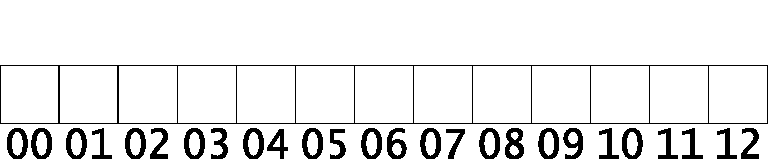
\includegraphics[width=\linewidth]{images/free}
\end{frame}

\begin{frame}[fragile]{»Dinge« und Speicher}
	Alle Definitionen legen »Dinge« an.\\
	{\tiny Ausnahme: \verb|static|}
	
	{\footnotesize
	\begin{block}{}
		\lstinputlisting[language=C++, linerange={3-4, 6-6}]{cpp-code/objects.cpp}
	\end{block}
	}
	
	\pause
	\vspace{1em}
	
	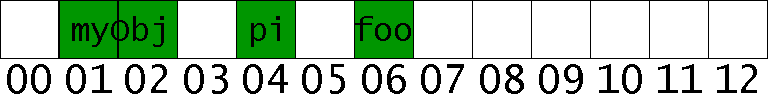
\includegraphics[width=\linewidth]{images/object_things}
\end{frame}


\subsection{Referenzen}

\begin{frame}[fragile]{Referenz: Referenzen}
	\verb|TYPE& add\_name = orig\_name;|
	\begin{itemize}
		\item Führt \verb|add_name| als zusätzlichen Namen für das »Ding« mit dem Namen \verb|orig_name| ein.
		\item \verb|add_name| heißt auch eine Referenz auf \verb|orig_name|.
	\end{itemize}
	
	\vspace{2em}
	
	Achtung: Eine Referenz muss immer gleich »initialisiert« werden, d.h. mittels \verb|=| einem »Ding« zugeordnet. {\tiny Bei Klassen-Membern in der Initialisations-Liste des Konstruktors.}
\end{frame}

\begin{frame}[fragile]{»Dinge« und Referenzen}
	Eine Referenz ist ein zusätzlicher Namen für \emph{dasselbe} »Ding«.\\
	Die Speicherdauer wird dadurch \emph{nicht} beeinflusst.
	
	{\footnotesize
	\begin{block}{}
		\lstinputlisting[language=C++, linerange=14-15]{cpp-code/objects.cpp}
	\end{block}
	}
	
	\pause
	
	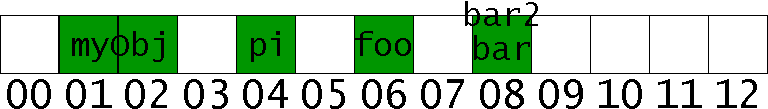
\includegraphics[width=\linewidth]{images/object_refs}
	
	\pause
	
	{\footnotesize
	\begin{block}{}
		\lstinputlisting[language=C++, linerange=16-17]{cpp-code/objects.cpp}
	\end{block}
	}
\end{frame}

\begin{frame}[fragile]{Referenzen als Parameter}
	Nutzt man eine Referenz als Parameter, so kann man innerhalb der Funktion den Wert des übergebenen »Dings« ändern:
	
	{\footnotesize
	\begin{block}{}
		\lstinputlisting[language=C++, linerange=34-38]{cpp-code/objects.cpp}
	\end{block}
	}
	
	\pause
	
	{\footnotesize
	\begin{block}{}
		\lstinputlisting[language=C++, linerange=19-22]{cpp-code/objects.cpp}
	\end{block}
	}
\end{frame}


\subsection{Pointer}

\begin{frame}[fragile]{Adressen und Pointer}
	Jedes Byte hat eine eindeutige Adresse.
	
	Man darf keine Annahmen darüber treffen, wie diese Adresse tatsächlich aussieht oder wie groß sie ist!
	Was man tun darf, sind Operationen mit \emph{Pointern}. Pointer sind Container von Adressen.
	
	\pause
	\vspace{1em}
	
	Wir wollen jedoch zwecks Anschauung eine Adresse mit der Nummer \emph{der} Bytes eines »Dings« identifizieren.
	
	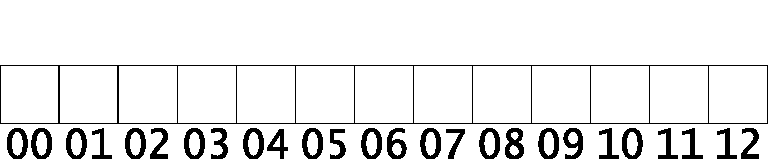
\includegraphics[width=\linewidth]{images/free}
\end{frame}

\begin{frame}[fragile]{»Dinge« und Pointer}
	Sei \verb|NAME| der Name eines »Dings«. Mit \verb|&NAME| erhalte ich dann die Adresse des »Dings«. Die Adresse selbst ist auch wieder ein »Ding«!
	
	\vspace{1em}
	\pause
	
	Als »Ding« hat die Adresse einen Typ:
	{\footnotesize
	\begin{block}{}
		\lstinputlisting[language=C++, linerange=24-25]{cpp-code/objects.cpp}
	\end{block}
	}
	
	\pause
	
	Das »Ding« \verb|NAME| habe den Typen \verb|TYPE|. Dann hat die Adresse des »Dings« den Typ \verb|TYPE*|.
\end{frame}


\begin{frame}[fragile]{»Dinge«, Pointer und Adressen}
	Ein Beispiel:
	
	{\footnotesize
	\begin{block}{}
		\lstinputlisting[language=C++, linerange={3-4, 6-6}]{cpp-code/objects.cpp}
	\end{block}
	}
	
	\vspace{1em}
	\phantom{
		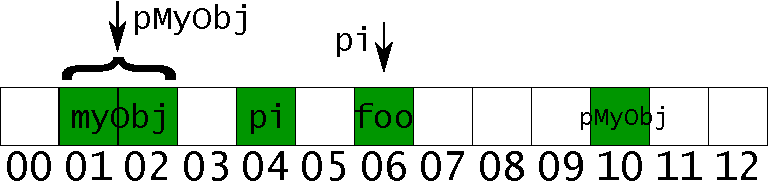
\includegraphics[width=\linewidth]{images/object_points_addr}
	}
\end{frame}

	\begin{frame}[fragile]{»Dinge«, Pointer und Adressen}
		Ein Beispiel:
		
		{\footnotesize
		\begin{block}{}
			\lstinputlisting[language=C++, linerange={3-4, 6-6, 10-10}]{cpp-code/objects.cpp}
		\end{block}
		}
		
		\vspace{1em}
		\phantom{
			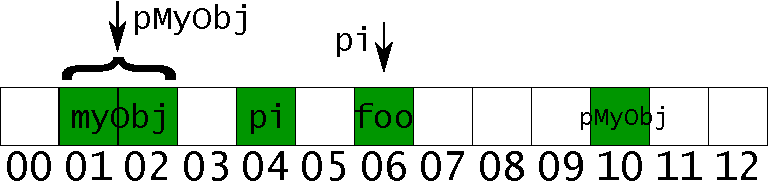
\includegraphics[width=\linewidth]{images/object_points_addr}
		}
	\end{frame}

	\begin{frame}[fragile]{»Dinge«, Pointer und Adressen}
		Ein Beispiel:
		
		{\footnotesize
		\begin{block}{}
			\lstinputlisting[language=C++, linerange={3-4, 6-6, 10-10, 27-27}]{cpp-code/objects.cpp}
		\end{block}
		}
		
		\pause
		\vspace{1em}
		
		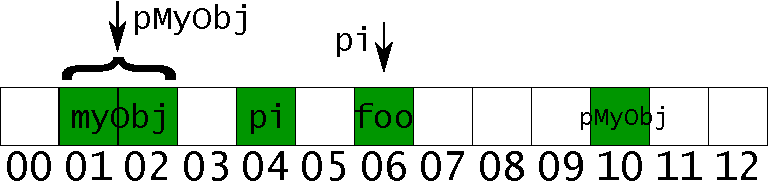
\includegraphics[width=\linewidth]{images/object_points_addr}
	\end{frame}


\begin{frame}[fragile]{Pointer vs. Referenzen}
	\footnotesize
	\begin{tabular}{c|c}
		Pointer & Referenz \\ \hline
		ist ein »Ding« & ist nur ein zusätzlicher Name \\
		enthält eine Adresse & enthält selbst nichts \\
		Inhalt kann sich ändern & bezieht sich immer auf dasselbe »Ding« \\
		Inhalt muss nicht sinnvoll sein & bezieht sich auf ein existierendes »Ding« \\
	\end{tabular}
	
	\pause
	
	{\footnotesize
	\begin{block}{}
		\lstinputlisting[language=C++, linerange={4-4, 27-31}]{cpp-code/objects.cpp}
	\end{block}
	}
\end{frame}

\section{C++ und der Speicher}


\begin{frame}{Von-Neumann-Architektur}
	Aus: \url{de.wikipedia.org/wiki/Von-Neumann-Architektur}
	
	\begin{block}{Komponenten der Von-Neumann-Architektur}
		\begin{itemize}
			\item CPU (vereinfacht)
			\item Speicher mit wahlfreiem Zugriff und linearem Adressraum (RAM)
			\item Ein-/Ausgabewerk bzw. \emph{anderes Zeug} (Festplatte, Netzwerk, Bildausgabe, Uhrzeit, \dots)
		\end{itemize}
	\end{block}
	
	\pause
	
	C++ selbst ermöglicht nur -- und eingeschränkte! -- Verwendung der CPU und des Speichers. Bis auf wenige Ausnahmen müssen alle anderen Komponenten über das \emph{Betriebssystem} mittels \emph{Application Binary Interfaces} angesprochen werden.
\end{frame}

\begin{frame}{Programm \& Programmablauf}
	\footnotesize
	
	\begin{block}{Das Programm ist gespeichert (und nicht gelötet)}
		\begin{itemize}
			\item Die Befehle des Programms sind im RAM gespeichert.
			\item Die Daten, auf welche das Programm zugreifen kann, sind ebenfalls im RAM gespeichert.
			\item Es gibt einen \emph{instruction pointer}, der auf den nächst auszuführenden Befehl zeigt (= dessen Adresse enthält).
		\end{itemize}
	\end{block}
	
	\pause
	
	\begin{block}{Das Programm wird sequentiell (schrittweise) ausgeführt}
		\begin{itemize}
			\item Der nächste Befehl wird mittels des \emph{instruction pointers} gelesen und ausgeführt.
			\item Normalerweise wird anschließend der \emph{instruction pointer} um Eins erhöht ($\implies$ die Befehle stehen »nacheinander« im RAM).
			\item Es gibt Sprung-Befehle und von einer Bedingung abhängige Sprung-Befehle, die den \emph{instruction pointer} auf einen anderen Wert setzen können.
		\end{itemize}
	\end{block}
\end{frame}

\begin{frame}[fragile]{Implementierung in C++}
	\footnotesize
	
	\begin{block}{Speicher mit linearem Adressraum}
		\begin{lstlisting}[language=C++]
			int i;
			i = 5;

			int* pi;
			pi = &i;
		\end{lstlisting}
	\end{block}
	
	\pause
	
	\begin{block}{Instruction Pointer und Sprungbefehle}
		\begin{lstlisting}[language=C++]
			int i;
			cin >> i;

			if(42 == i)
			    cout << "It's the solution!" << endl;
			else
			    cout << "It's NOT the solution!" << endl;
		\end{lstlisting}
	\end{block}
\end{frame}

\begin{frame}{Kurz: Datenstruktur}
	\begin{itemize}
		\item Wir haben linearen Speicher.
		\item Wir haben meist nicht nur ein Datum, sondern viele Daten, die miteinander in Verbindung stehen.
		\item Die Datenstruktur definiert (1), wie die Daten abgelegt und organisiert sind/werden (\emph{Implementierung} einer Datenstruktur).
		\item Die Datenstruktur definiert (2) die Art und Weise, wie auf die Daten zugegriffen werden kann (\emph{Interface} der Datenstruktur).
	\end{itemize}
	
	\pause
	
	\footnotesize
	
	\begin{block}{Einfachstes Beispiel: Array}
		\emph{Implementierung}: Daten sind sequentiell im Speicher abgelegt
		
		\emph{Interface}:
		\begin{itemize}
			\item Zugriff auf jedes beliebige Element des Arrays anhand seiner eindeutigen Nummer ($\in \mathbb{N}_0$).
			\item Die Nummern sind fortlaufend und beginnen bei 0, sie ändern sich nicht.
			\item Von jedem Element gelangt man zu jedem anderen beliebigen Element des Arrays.
		\end{itemize}
	\end{block}
\end{frame}

\begin{frame}{Stack}
	Analogie: Ein Stapel Karten (ich lege eine Karte obenauf oder nehme sie weg).
	
	\hspace{1em}
	\pause
	
	\emph{Implementierung}:
	\begin{itemize}
		\item Ein fester, zuvor angelegter Speicherblock (Array).
		\item Ein Stack-Pointer, der eine Adresse auf dem Stack speichert. Zu Beginn zeigt dieser auf die höchste Adresse im Speicherblock.
		\item Beim Einfügen (Entfernen) von Elementen wird der Stack-Pointer erniedrigt (erhöht).
	\end{itemize}
	
	\pause
	
	\emph{Interface}:
	\begin{itemize}
		\item Einfügen eines Elements beliebiger Größe {\tiny(es muss natürlich in den verbleibenden freien Speicher des Stacks passen)} an das Ende des Stacks (\enquote{auf den Stapel legen}).
		\item Zugriff auf das zuletzt eingefügte Element.
		\item Entfernen des zuletzt eingefügten Elements.
	\end{itemize}
\end{frame}

\begin{frame}[fragile]{\enquote{Stack-Variablen}, automatic storage duration}
	\footnotesize

	Die Definition eines »Dings« legt dieses (den Speicher!) auf den Stack des Programms {\tiny Ausnahme: \verb|static|}.
	\begin{block}{}
		\begin{lstlisting}[language=C++]
			int foo;
			double bar;
			bool marvin = false;
			MyClass myObject;
			ofstream myOutputFileStream("C:/log.txt");
		\end{lstlisting}
	\end{block}
	
	\pause
	
	Am Ende des Blocks, in welchem das »Ding« erzeugt wurde (der \emph{scope} der Variablen endet), wird es vom Stack genommen:
	\begin{block}{}
		\begin{lstlisting}[language=C++]
			{
			    int foo;
			}
		\end{lstlisting}
	\end{block}
\end{frame}

\begin{frame}[fragile]{Namen und Blöcke}
	Normalerweise darf und kann ich auf die Namen aller übergeordneten Blöcke zugreifen.
	{\scriptsize Ausnahme: Sobald ein neuer Block beginnt, darf ich einen Namen neu verwenden und damit die alte Verwendung überdecken.}
	
	\begin{block}{}
		\begin{lstlisting}[language=C++]
			int foo = 42;
			{
			    int bar = foo;
			    int foo = 44;
			}
		\end{lstlisting}
	\end{block}
\end{frame}

\begin{frame}[fragile]{Namen und Funktionen}
	\footnotesize
	
	Da Funktionen von überall her aus aufgerufen werden können, dürfen innerhalb von Funktionen keine Namen von »übergeordneten« Blöcken verwendet werden.
	
	\scriptsize
	\begin{block}{}
		\begin{lstlisting}[language=C++]
			void foobar() {
			    // ++bar;    // VERBOTEN!
			    int foo = 42;
			    ...
			    foobar();
			}
			
			int barfoos() {
			    int bar = 0;
			    foobar();
			}
			
			int main() {
			    foobar();
			}
		\end{lstlisting}
	\end{block}
\end{frame}

\begin{frame}[fragile]{Stack-Frame (1)}
	Scope, Blöcke, Namen usw. basieren auf dem Prinzip des \emph{Stack-Frames}.
	
	\pause
	
	\begin{block}{Stack-Frame}
		\begin{itemize}
			\item Jeder Block \verb|{ ... }| bildet einen \emph{Stack-Frame}.
			\item Zu Beginn des Stack-Frames werden alle im Block definierten »Dinge« auf den Stack gelegt.
			\item Nach Ende des Frames werden sie vom Stack genommen.
			\item Die Reihenfolge auf dem Stack entspricht der Reihenfolge der Definition {\tiny(abgesehen von Optimierungen)}.
		\end{itemize}
	\end{block}
	
	\pause
	
	Der Stack-Pointer zu Beginn des Stack-Frames wird gespeichert und nennt sich Frame-Pointer (oder Base-Pointer).
\end{frame}

\begin{frame}[fragile]{Zugriff auf \enquote{Stack-Variablen}}
	Der Stack an sich erlaubt nur den Zugriff auf das zuletzt eingefügte Element. ABER:
	\pause
	\begin{itemize}
		\item Der Stack ist implementiert als ein Array plus einem Pointer.
		\item In einem Array kann man auf jedes beliebige Element zugreifen!
		\item Ein Variablen-Name in C++ wird daher durch einen \emph{festen} Offset vom Frame-Pointer ersetzt.
	\end{itemize}
	
	\pause
	
	\footnotesize
	\begin{block}{}
		\begin{lstlisting}[language=C++]
			//- Annahme *hier*: Stack-Pointer esp = 40
			{   //- Frame-Pointer ebp := esp, hier: 40
			    //- esp := esp - sizeof(foo) - sizeof(bar), hier: 32
			    int foo;    // Tut hier nichts!
			    foo = 42;   // foo entspricht ebp - 0 = ebp, hier: 40
			    int bar;    // Tut hier nichts!
			    bar = 21;   // bar entspricht ebp - sizeof(int), hier: 36
			}   //- esp := ebp, hier: 40
		\end{lstlisting}
	\end{block}
\end{frame}

\begin{frame}[fragile]{Grenzen des Stacks}
	\begin{itemize}
		\item Für den Stack wird \emph{einmalig} eine feste Menge zusamenhängender Speicher zur Verfügung gestellt.
		\item Der Speicher für alle Variablen innerhalb eines Blocks wird zu Beginn des Blocks alloziert.
		\item Die Variablen-Namen entsprechen \emph{festen} Offsets vom ebp.
	\end{itemize}
	
	\pause
	
	\begin{itemize}
		\item Problem 1: Wie alloziere ich Speicher für eine sehr große Menge Daten?
		\item Problem 2: Wie alloziere ich eine zur Laufzeit festgelegte Menge Speicher?
		\item Problem 3: Wie verwende ich Daten in anderen Stack-Frames (Funktionen usw.)?
	\end{itemize}
	
	\pause
	
	\tiny
	Detail:
	Ich kann genau \emph{einmal} innerhalb eines Blocks eine dynamische, d.h. zur Laufzeit festgelegte, Menge Speicher allozieren;
	und zwar \emph{nachdem der Speicher aller \enquote{Stack-Variablen} des Blocks alloziert wurde}.
	
	Das ist allerdings hässlich und nicht standardisiert!
	Resultat: Ich kann in Standard-C++ \emph{gar nicht} eine dynamische Menge Speicher auf dem Stack allozieren!
\end{frame}

\begin{frame}{Heap}
	Für die Schwächen und Unzulänglichkeiten des Stacks / automatic storage duration benötigt man eine andere Datenstruktur zur Speicherverwaltung.
	Diese kann ein Heap sein.
	
	\pause
	
	\begin{block}{Heap}
		\emph{Implementierung}: Magie!
		
		\pause
		
		\emph{Interface}:
		\begin{itemize}
			\item Einfügen eines Elements beliebiger Größe, \emph{keine Garantien über die Adresse des allozierten Speichers!}.
			\item Entfernen eines beliebigen Elements.
			\item Die Adressen eines Elements ändert sich \emph{nicht} wenn man andere Elemente einfügt oder entfernt.
		\end{itemize}
	\end{block}
\end{frame}

\begin{frame}[fragile]{Allokation auf dem Heap}
	\verb|new TYPE;| \hspace{1em} bzw. \hspace{1em} \verb|new TYPE(PARAMETER);|
	\begin{itemize}
		\item Alloziert das »Ding« auf dem Heap (den Speicher!).
		\item Ruft den Konstruktor von TYPE auf (und übergibt die PARAMETER).
		\item Gibt die Adresse des Speichers zurück, als \verb|TYPE*|.
	\end{itemize}
	
	\vspace{2em}
	
	\verb|new TYPE[DYNAMIC_NUMBER];| -- die Variante mit Parametern \emph{existiert nicht!}
	\begin{itemize}
		\item Alloziert \verb|DYNAMIC_NUMBER| »Dinge« auf dem Heap (den Speicher!).
		\item Ruft für jedes Element den \emph{default}-Konstruktor von TYPE auf.
		\item Gibt die Adresse des Speichers des nullten Elements zurück, als \verb|TYPE*|.
	\end{itemize}
\end{frame}

\begin{frame}[fragile]{\enquote{Heap-Variablen}}
	Da die Adresse eines »Dings« auf dem Heap erst zur Laufzeit festgelegt wird, kann der Compiler nicht wie bei Stack-Variablen mit festen Werten (Offsets) arbeiten.
	
	\hspace{1em}
	\pause
	
	Man arbeitet stattdessen mit zwei Schritten:
	\begin{itemize}
		\item Man speichert auf dem Stack die Adresse der Heap-Variablen.
		\item Man lädt von der Adresse \emph{selbst} den Wert des Heap-»Dings« $\Rightarrow$ \emph{dereferenzieren}
	\end{itemize}
	\pause
	
	\footnotesize
	\begin{block}{}
		\begin{lstlisting}[language=C++]
			int* p;         // Stack-Variable
			p = new int;    // Speichere in p die Adresse des Heap->Dings<.
			cout << *p;     // Lade von der Adresse in p den Wert, Ausgabe.
		\end{lstlisting}
	\end{block}
\end{frame}

\begin{frame}[fragile]{dynamic storage duration}
	Da C++ / der Compiler nur die Addresse des Objekts hat, kann der Compiler nicht so einfach wie beim Stack die »Dinge« wegräumen:
	
	{\footnotesize
	\begin{block}{}
		\begin{lstlisting}[language=C++, escapechar=\%]
			int* p0 = 0;
			{
			    int* p = new int;
			    p0 = p;
			}
			%\phantom{...}%
			%\phantom{\Hilight delete p0;}%
		\end{lstlisting}
	\end{block}
	}
	
	Man muss sich daher selbst um das Aufräumen kümmern!
\end{frame}

\begin{frame}[fragile]{Deallokation vom Heap}
	\verb|delete ADDRESS;| -- ADDRESS muss eine Rückgabe von \verb|new| sein, sei hier vom Typ TYPE*
	\begin{itemize}
		\item Ruft den Destruktor vom Objekt auf (\verb|ADDRESS->~TYPE();|)
		\item Dealloziert den Speicher vom Heap.
	\end{itemize}
	
	\vspace{2em}
	
	\verb|delete[] ADDRESS;| -- ADDRESS muss eine Rückgabe von \verb|new [...]| sein
	\begin{itemize}
		\item Ruft nacheinander die Destruktoren der Elementes auf, beginnend mit dem letzten.
		\item Dealloziert den Speicher vom Heap.
	\end{itemize}
\end{frame}

\begin{frame}[fragile]{dynamic storage duration}
	Da C++ / der Compiler nur die Addresse des Objekts hat, kann der Compiler nicht so einfach wie beim Stack die »Dinge« wegräumen:
	
	{\footnotesize
	\begin{block}{}
		\begin{lstlisting}[language=C++, escapechar=\%]
			int* p0;
			{
			    int* p = new int;
			    p0 = p;
			}
			...
			%\Hilight%delete p0;
		\end{lstlisting}
	\end{block}
	}
	
	Man muss sich daher selbst um das Aufräumen kümmern!
\end{frame}

\section{Stack und Heap}

\subsection{»Dinge« und Stack}

\newcommand{\stackimgframe}[3]{
	\begin{frame}[t]{#1}
		\includegraphics[width=\linewidth]{images/#2}
		
		\begin{block}{}
			#3
		\end{block}
	\end{frame}
}

\begin{frame}[fragile]{Allokation auf Stack}
	\verb|TYPE name;| \hspace{1em} bzw. \hspace{1em} \verb|TYPE name(PARAMETER);|
	\begin{itemize}
		\item Alloziert das »Ding« vom Typ \verb|TYPE| auf dem Stack (den Speicher!).
		\item Ruft den Konstruktor von TYPE auf (und übergibt die PARAMETER).
		\item Führt den Namen \verb|name| für das »Ding« ein.
	\end{itemize}
	
	\vspace{2em}
	
	\verb|TYPE name[STATIC_NUMBER];| -- die Variante mit Parametern \emph{existiert nicht!}
	\begin{itemize}
		\item Alloziert \verb|STATIC_NUMBER| »Dinge« auf dem Stack (den Speicher!).
		\item Ruft für jedes Element den \emph{default}-Konstruktor von TYPE auf.
		\item Führt den Namen \verb|name| ein, dieser ist (fast) identisch zur Adresse des nullten Elements.
	\end{itemize}
\end{frame}

\stackimgframe{Leerer Speicher}{free}{}

\begin{frame}[fragile, t]{Alloziere einen Stack}
	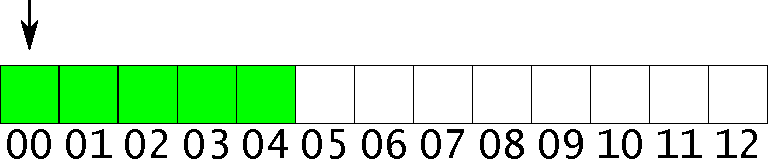
\includegraphics[width=\linewidth]{images/stack_frag_alloc}
	
	\begin{block}{}
		\lstinputlisting[language=C++, linerange=1-1]{cpp-code/objects.cpp}
	\end{block}
	
	Der Stack-Pointer (Pfeil) zeigt auf den nächsten freien Speicherblock.
\end{frame}

\begin{frame}[fragile, t]{Definition von »Dingen«}
	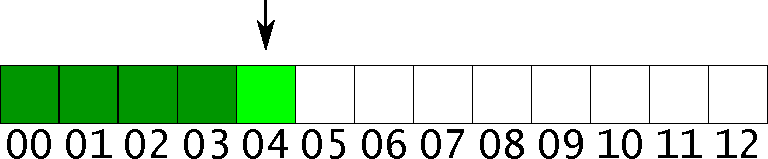
\includegraphics[width=\linewidth]{images/stack_frag_store}
	
	\vspace{1em}
	
	Alle Definitionen legen »Dinge« auf dem Stack an.\\
	{\tiny Ausnahme: \verb|static|}
	
	{\footnotesize
	\begin{block}{}
		\lstinputlisting[language=C++, linerange=3-6]{cpp-code/objects.cpp}
	\end{block}
	}
\end{frame}

\begin{frame}[fragile, t]{Direkter Zugriff auf »Dinge«}
	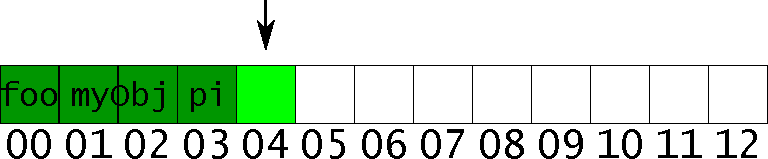
\includegraphics[width=\linewidth]{images/object_names}
	
	\vspace{1em}
	
	Der Compiler kann den Namen des »Dings« direkt verwenden, d.h. in einer Operation auf den Speicher zugreifen.
	
	{\footnotesize
	\begin{block}{}
		\lstinputlisting[language=C++, linerange=8-8]{cpp-code/objects.cpp}
	\end{block}
	}
\end{frame}

\begin{frame}[fragile, t]{Indirekter Zugriff auf »Dinge«}
	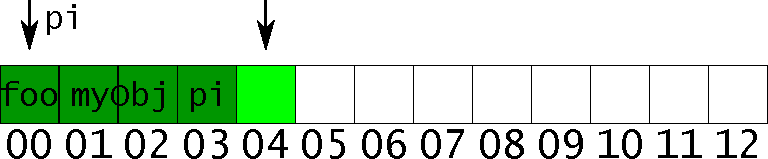
\includegraphics[width=\linewidth]{images/object_points}
	
	\vspace{1em}
	
	Pointer haben zum Inhalt die Adresse eines »Dings«.
	
	{\footnotesize
	\begin{block}{}
		\lstinputlisting[language=C++, linerange=10-10]{cpp-code/objects.cpp}
	\end{block}
	}
\end{frame}

\begin{frame}[fragile, t]{Entfernen von »Dingen«}
	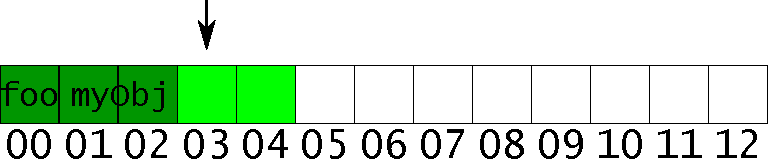
\includegraphics[width=\linewidth]{images/object_pop}
	
	\vspace{1em}
	
	Endet der Block, in welchem ein »Ding« definiert wurde, wird es weggeräumt.
	
	{\footnotesize
	\begin{block}{}
		\lstinputlisting[language=C++, linerange={5-6, 11-12}]{cpp-code/objects.cpp}
	\end{block}
	}
\end{frame}

\begin{frame}{Reihenfolge des Entfernens von »Dingen«}
	Aufgrund der Architektur des Stacks werden die »Dinge« in der Reihenfolge weggeräumt, in dem sie erzeugt wurden.
	
	\pause
	\vspace{1em}
	
	Weitere Besonderheit der Implementierung: Alle Speicherreservierungen im Blocks auf dem Stack können gleichzeitig vorgenommen werden, und zwar zu Beginn des Blocks.
\end{frame}


\subsection{Fragmentierung des Stacks?}

\stackimgframe{Leerer Speicher}{free}{}

\stackimgframe{Alloziere einen Stack}{stack_frag_alloc}{
	\lstinputlisting[language=C++, linerange=1-1]{cpp-code/stack.cpp}
}

\stackimgframe{Belege den Stack (push)}{stack_frag_store}{
	\lstinputlisting[language=C++, linerange=3-6]{cpp-code/stack.cpp}
}

\stackimgframe{Entferne vom Stack (pop)}{stack_frag_pop}{
	\lstinputlisting[language=C++, linerange=3-7]{cpp-code/stack.cpp}
}

\stackimgframe{Voller Stack}{stack_frag_pre_realloc}{}

\stackimgframe{Alloziere mehr Speicher für den Stack}{stack_frag_realloc}{}

\stackimgframe{Belege mehr Stack}{stack_frag_more_store}{}

\stackimgframe{Entferne vom Stack}{stack_frag_dealloc}{}

\stackimgframe{Fragmentierter Stack}{stack_frag_full}{}


\subsection{Heap}

\begin{frame}[fragile]{Allokation auf dem Heap}
	\verb|new TYPE;| \hspace{1em} bzw. \hspace{1em} \verb|new TYPE(PARAMETER);|
	\begin{itemize}
		\item Alloziert das »Ding« auf dem Heap (den Speicher!).
		\item Ruft den Konstruktor von TYPE auf (und übergibt die PARAMETER).
		\item Gibt die Adresse des Speichers zurück, als \verb|TYPE*|.
	\end{itemize}
	
	\vspace{2em}
	
	\verb|new TYPE[DYNAMIC_NUMBER];| -- die Variante mit Parametern \emph{existiert nicht!}
	\begin{itemize}
		\item Alloziert \verb|DYNAMIC_NUMBER| »Dinge« auf dem Heap (den Speicher!).
		\item Ruft für jedes Element den \emph{default}-Konstruktor von TYPE auf.
		\item Gibt die Adresse des Speichers des nullten Elements zurück, als \verb|TYPE*|.
	\end{itemize}
\end{frame}

\begin{frame}[fragile]{Deallokation vom Heap}
	\verb|delete ADDRESS;| -- ADDRESS muss eine Rückgabe von \verb|new| sein, sei hier vom Typ TYPE*
	\begin{itemize}
		\item Ruft den Dekonstruktor vom Objekt auf (\verb|ADDRESS->~TYPE();|)
		\item Dealloziert den Speicher vom Heap.
	\end{itemize}
	
	\vspace{2em}
	
	\verb|delete[] ADDRESS;| -- ADDRESS muss eine Rückgabe von \verb|new [...]| sein
	\begin{itemize}
		\item Ruft den Dekonstruktor jedes Elementes auf.
		\item Dealloziert den Speicher vom Heap.
	\end{itemize}
\end{frame}

\stackimgframe{Leerer Speicher}{free}{}

\stackimgframe{Alloziere einen Stack fester Größe}{stack_heap_alloc}{
	\lstinputlisting[language=C++, linerange=1-1]{cpp-code/stack.cpp}
}

\stackimgframe{Belege den Stack}{stack_heap_store}{
	\lstinputlisting[language=C++, linerange=14-16]{cpp-code/stack.cpp}
}

\stackimgframe{Alloziere auf dem Heap}{stack_heap_alloc_plusheap}{
	\lstinputlisting[language=C++, linerange=18-21]{cpp-code/stack.cpp}
}

\stackimgframe{Fragmentierter Heap}{stack_heap_frag}{
	\lstinputlisting[language=C++, linerange=23-25]{cpp-code/stack.cpp}
}

\stackimgframe{Defragmentierter Heap}{stack_heap_defrag}{
	\lstinputlisting[language=C++, linerange=23-26]{cpp-code/stack.cpp}
}

\begin{frame}[fragile]{Storage duration}
	Der C++ Standard kennt weder Stack noch Heap, dafür aber eine \emph{Speicherdauer der »Dinge«} (storage duration of objects).
	
	\vspace{1em}
	
	\begin{block}{automatic storage duration}
		Das »Ding« wird bei der Definition angelegt und beim Ende des Blocks weggeräumt $\rightarrow$ Stack
	\end{block}
	
	\vspace{1em}
	
	\begin{block}{dynamic storage duration}
		Man muss das »Ding« selbst erzeugen (\verb|new|) und selbst wegräumen (\verb|delete|).
	\end{block}
\end{frame}

\begin{frame}[fragile]{Stack vs. Heap}
	\begin{block}{Stack}
		\begin{itemize}
			\item Schnelle Allokation \& Deallokation {\tiny(z.B. ein einzige Operation für beliebig viel »Dinge«!)}
			\item Direkter, schneller Zugriff
			\item Optimierungen gut und einfach(er) für den Compiler
			\item Erzeugung \& Aufräumen ist automatisch
			\item Begrenzter Speicher (z.B. 1~MB auf Desktop-Rechner)
			\item Größe des »Dings« und Anzahl muss dem Compiler bekannt sein
		\end{itemize}
	\end{block}
	
	\begin{block}{Heap}
		\begin{itemize}
			\item Für große »Dinge«
			\item Eigene Verwaltung der Speicherdauer
			\item Speicherverwaltung während das Programm läuft
		\end{itemize}
	\end{block}
\end{frame}



\end{document}
